% éèàùôê

\chapter{Les mobiles de Choco}
\label{chapitre:choco}

%%%%%%%%%%%%%%%%%%%%%%%%%%%%%%%%%%%%%%%%%%%%%%%%%%%%%%%%%%%%%%%%%%%%%%%%%%%%%%%%
%                                    TP 5                                      %
%%%%%%%%%%%%%%%%%%%%%%%%%%%%%%%%%%%%%%%%%%%%%%%%%%%%%%%%%%%%%%%%%%%%%%%%%%%%%%%%

\section{Des contraintes sans \prolog{}}

Les problèmes concrets de l'industrie utilisant les contraintes ne sont pas
souvent résolus entièrement en \prolog{}. Il existe alors plusieurs solutions pour
utiliser vos connaissances en programmation par contraintes :

\begin{itemize}

\item utiliser une interface entre \prolog{} et le langage utilisé dans le reste
      du projet (par exemple ECLiPSe s'interface très bien avec JAVA et C++)~;

\item utiliser un autre moteur de résolution des contraintes (i.e. un autre
      solveur) dans un autre langage. 

\end{itemize}

C'est cette dernière solution que nous allons explorer dans ce chapitre. Il
existe beaucoup de moteurs dans différents langages, pour n'en citer que
quelques uns :

\begin{itemize}
	\item en C++ : Disolver, gecode, \ldots
	\item en Java : JaCob, JCK, JCL, Choco, \ldots
	\item en Ocaml : FaCiLe, \ldots
\end{itemize}

Nous allons utiliser \textbf{Choco} pour résoudre un problème simple dans le
domaine des entiers dans un programme Java. Vous trouverez en annexe
\ref{annexe:choco} un descriptif des fonctionnalités de Choco pour poser et
résoudre les problèmes. Vous pouvez aussi aller voir sur le site de Choco
\url{http://www.emn.fr/z-info/choco-solver/index.html}. 

Nous vous fournissons une grosse partie du code Java, il ne reste que
la partie programmation des contraintes à réaliser. Ce code est fourni
à l'emplacement \url{/home-info/commun/4info/Contraintes_choco} de
votre machine.

\section{Le problème : équilibrer un mobile}

Le problème que nous considérons est l'équilibrage d'un mobile de structure
fixée décrite par la figure \ref{fig:mobile} (il n'est pas demandé de résoudre
le problème dans le cas général, même si la programmation objet de Java le
permettrait facilement).

\begin{figure}
\begin{center}
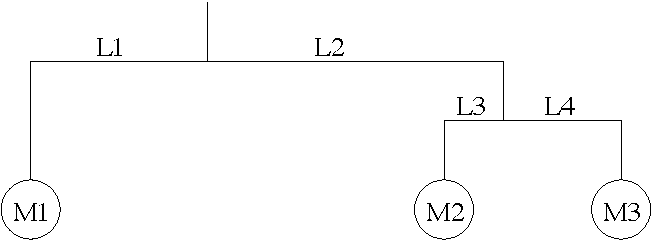
\includegraphics[width=10cm]{mobile.pdf}
\caption{Le mobile à équilibrer}
\label{fig:mobile}
\end{center}
\end{figure}

Le problème comporte donc 7 variables entières (problème dans le domaine fini) :

\begin{itemize}

\item les longueurs des branches : L1 et L2 pour le premier étage et L3 et L4
      pour le second ;

\item les masses M1, M2 et M3 au bout des branches.

\end{itemize}

Le mobile est soumis à quelques contraintes (physiques). Le mobile doit pouvoir
tourner (une contrainte entre les longueurs à valeurs entières) sachant que les
masses sont de tailles négligeables. Le mobile doit être équilibré (ce qui
correspond à deux contraintes entre les variables). Pour équilibrer le mobile
on dispose de 20 masses différentes, dont les poids à valeur entière
s'échantillonnent de 1 à 20g.

\section{Les problèmes à résoudre}

\begin{question}
Écrire les programmes qui résolvent les deux problèmes qui suivent.
\end{question}

\begin{enumerate}
\item L'utilisateur entre des valeurs pour les longueurs des branches, vous
      devez vérifier que ces longueurs sont cohérentes ;

\item Trouver les masses M1, M2 et M3 qu'il faut choisir parmi les poids
      disponibles pour équilibrer les mobiles (ce qui n'est pas toujours
      possible mais parfois il existe plusieurs solutions).

\end{enumerate}

Il faut définir les variables et leurs domaines puis poser les différentes
contraintes. Il vous sera indiqué en TP quelles méthodes Java compléter.
